% GENERATED FROM typst/manual/sections/07_galactic_lensing_plan.typ BY scripts/typ2tex.py (v1.0.0) — DO NOT EDIT.
% Edit canonical Typst under typst/ and regenerate with: python3 scripts/typ2tex.py --root . --outdir latex

\section{Galactic Lensing Diagnostic Plan}\label{manual:galactic-lensing-diagnostic-plan}

\paragraph{Calculation card.}
Toy bins, SPARC medium proxies, SWELLS targets and L3 input requirements have
separate roles. The inline aggregate tables retain their historical results;
per-system inputs, cohort membership, exclusions and evaluator/gate lineage
are still needed for replay. Shared target reductions and uncertainty enter
one joint comparison under \secref{manual:calculation-spine}, not additional
independent medium evidence. The L3 gate below states the missing stages.

\aodnoteblock{Scope}{This section applies the current A$\Omega$D field-ring and $\delta_3$ notation to a staged galactic-lensing diagnostic plan. It is a manual/application plan with an explicit L3 data-package gate.}

\aodprovenance{\mainsection{main:subsec:fractal-field-ring-gate};
\mainsection{main:sec:field-dynamics};
\secref{manual:cross-return-short-window};
\secref{manual:prediction-test-registry}.}

\aodliteraturenote{SWELLS target lane: Treu et al.~\cite{treu-swells-2011}, Brewer et al.~\cite{brewer-swells-2012}.}

\subsection{Lensing lanes}\label{manual:lensing-status-lock}

\begin{table}[H]
\centering
\caption{Galactic lensing diagnostic lanes.}
\label{tab:manual-lensing-status-lock}
{\footnotesize
\begin{tabular}{>{\raggedright\arraybackslash}p{0.240\linewidth}>{\raggedright\arraybackslash}p{0.100\linewidth}>{\raggedright\arraybackslash}p{0.560\linewidth}}
\toprule
Lane & Class & Active fields \\
\midrule
Toy 1 & L0 & exact internal $\delta_3$ fixture \\
SPARC5 & L1 & radial lens-medium data-support class; lens target fields are carried by SWELLS or L3 rows \\
SWELLS K0 & L2 & target acquisition \\
SWELLS K1 & L1/L2 & retained baseline \\
SWELLS K2/K3 & L1/L2 & audit diagnostics \\
K4 & L3 & higher-resolution lensing input-manifest row \\
L3 lensing input package & L3 & L3 input-manifest row; required fields: independent 3D medium fields, time-flow inputs, radiation-current gates, target-side quarantine, null controls, and audit \\
\bottomrule
\end{tabular}
}
\end{table}

\subsection{Field-ring spine}\label{manual:lensing-field-ring-spine}

The lensing fixture uses a discrete exoshedding field-ring calculation. The value table records the evaluated gate values.

\[
B_{\mathrm{lens}}=(\partial_TF_{\mathrm{exo}},\omega_{\mathrm{lens}}).
\]

\[
T^0_k=\sum_iS^{(i)}_k.
\]

\[
T^{\times}_k=T^0_k+\sum_{(i,j)\in E_{\mathrm{return}}}C^{\times}_{ij,k}(B_{\mathrm{lens}}).
\]

\[
T^{\times}_k-T^0_k=\sum_{(i,j)\in E_{\mathrm{return}}}C^{\times}_{ij,k}(B_{\mathrm{lens}}).
\]

\[
\Delta^{\mathbb{Z}}_k=T^{\times}_k-O_k,\qquad\delta_{3,k}(T^{\times},O)=(s^{(3)}_k,m_k),\qquad m_k=|\Delta^{\mathbb{Z}}_k|.
\]

\[
\delta_3(T^{\times},O)=(\delta_{3,k})_{k\in K}.
\]

\begin{figure}[H]
\centering
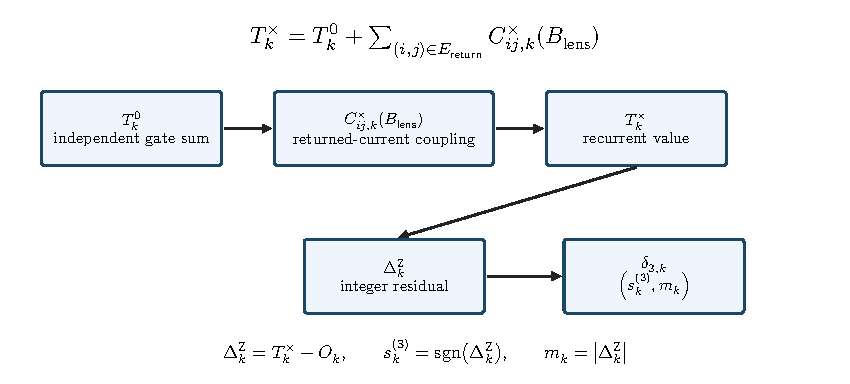
\includegraphics[width=0.92\linewidth,height=0.78\textheight,keepaspectratio]{figures/generated/lensing-02-frg-value-identity-delta3.pdf}
\caption{FRG value identity and $\delta_3$ audit. Gate values $T^0$, $C^{\times}$, and $T^{\times}$ are computed before the fixture comparator joins.}
\label{fig:manual-lensing-frg-delta3}
\end{figure}

\subsection{Toy fixture lane}\label{manual:lensing-toy-fixture-lane}

Toy 1 is the exact internal lensing toy. It belongs to the manual fixture lane and registry.

\begin{table}[H]
\centering
\caption{Toy 1 exact internal $\delta_3$ fixture summary.}
\label{tab:manual-lensing-toy-summary}
{\footnotesize
\begin{tabularx}{\linewidth}{>{\raggedright\arraybackslash}p{0.360\linewidth}r}
\toprule
Quantity & Value \\
\midrule
gates & 16 \\
target bins & 13 \\
events & 18 \\
caustic bins & 0, 2 \\
$\delta_3$ total $m$ & 0 \\
checks passed & 11/11 \\
\bottomrule
\end{tabularx}
}
\end{table}

\begin{figure}[H]
\centering
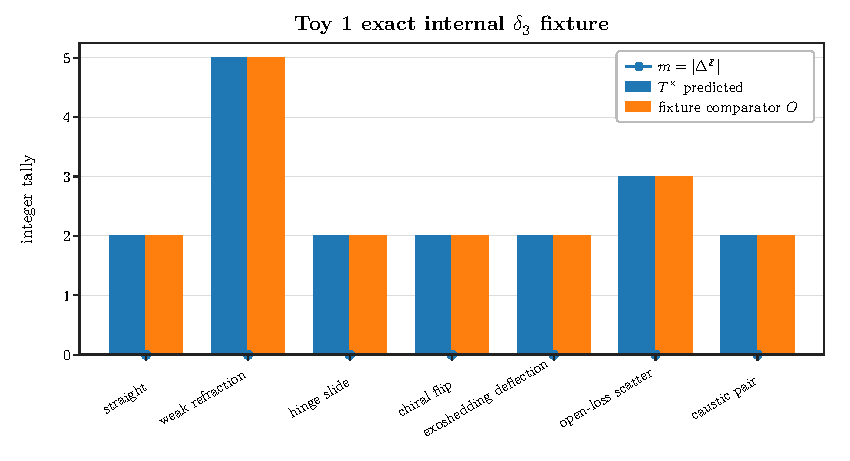
\includegraphics[width=0.92\linewidth,height=0.78\textheight,keepaspectratio]{figures/generated/lensing-01-toy1-delta3-class-tallies.pdf}
\caption{Toy 1 exact internal $\delta_3$ class tallies.}
\label{fig:manual-lensing-toy-delta3}
\end{figure}

\subsection{SPARC5 lens-medium diagnostic}\label{manual:lensing-sparc5-medium-diagnostic}

SPARC5 instantiates a radial lens-medium data-support class. It supplies radial field-medium inputs for diagnostic runs. Image-count, Einstein-radius, image-position, and shear target fields are target-side quantities carried by SWELLS or an L3 input package.

% GENERATED FROM typst/manual/tables/sparc5_medium_diagnostic_summary_table.typ BY scripts/typ2tex.py (v1.0.0) — DO NOT EDIT.
% Edit canonical Typst under typst/ and regenerate with: python3 scripts/typ2tex.py --root . --outdir latex

\begin{table}[H]
\centering
\caption{SPARC5 lens-medium summary.}
\label{tab:manual-lensing-sparc5-summary}
{\footnotesize
\begin{tabular}{>{\raggedright\arraybackslash}p{0.095\linewidth}>{\raggedright\arraybackslash}p{0.050\linewidth}>{\raggedright\arraybackslash}p{0.050\linewidth}>{\raggedright\arraybackslash}p{0.057\linewidth}>{\raggedright\arraybackslash}p{0.057\linewidth}>{\raggedright\arraybackslash}p{0.095\linewidth}>{\raggedright\arraybackslash}p{0.086\linewidth}>{\raggedright\arraybackslash}p{0.171\linewidth}>{\raggedright\arraybackslash}p{0.143\linewidth}}
\toprule
Galaxy & Bins & Gates & Events & Caustic & Median $|\Delta A_{\gamma}|$ & Max $|\Delta A_{\gamma}|$ & Dominant class & Status \\
\midrule
NGC2403 & 73 & 32 & 44 & 12 & 1.1667 & 1.9 & exoshedding deflection & lens-medium \\
NGC3198 & 43 & 32 & 44 & 12 & 1.2721 & 2.0 & exoshedding deflection & lens-medium \\
NGC6503 & 31 & 32 & 44 & 12 & 1.3801 & 2.4706 & exoshedding deflection & lens-medium \\
NGC2841 & 50 & 32 & 41 & 9 & 1.2416 & 1.7647 & exoshedding deflection & lens-medium \\
DDO154 & 12 & 32 & 46 & 14 & 1.2941 & 2.625 & exoshedding deflection & lens-medium \\
\bottomrule
\end{tabular}
}
\end{table}


\begin{figure}[H]
\centering
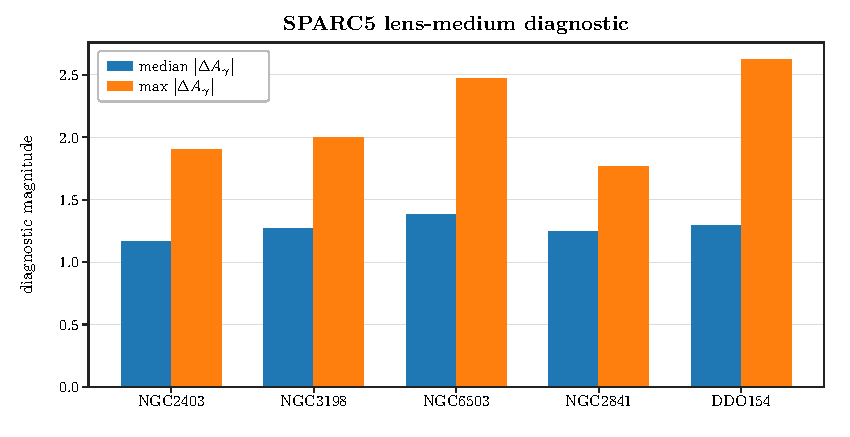
\includegraphics[width=0.92\linewidth,height=0.78\textheight,keepaspectratio]{figures/generated/lensing-03-sparc5-lens-medium-phase-proxy.pdf}
\caption{SPARC5 radial lens-medium data-support class. The plotted quantities are diagnostic medium proxies; lensing targets are carried by SWELLS or a higher-resolution class.}
\label{fig:manual-lensing-sparc5-proxy}
\end{figure}

\begin{figure}[H]
\centering
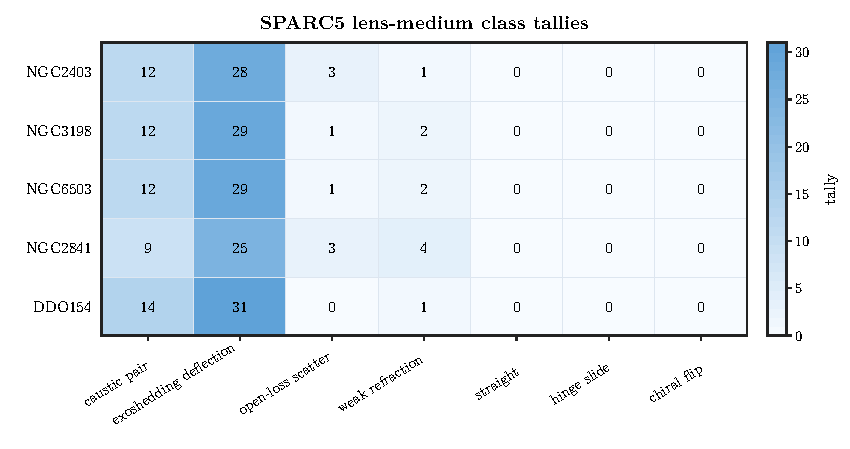
\includegraphics[width=0.92\linewidth,height=0.78\textheight,keepaspectratio]{figures/generated/lensing-04-sparc5-class-tally-heatmap.pdf}
\caption{SPARC5 lens-medium class tallies. The dominant diagnostic route class is recorded for audit.}
\label{fig:manual-lensing-sparc5-classes}
\end{figure}

\subsection{SWELLS target lane}\label{manual:lensing-swells-lane}

SWELLS supplies target-side acquisition fields for the lensing lane.

% GENERATED FROM typst/manual/tables/swells_k0_target_tallies_table.typ BY scripts/typ2tex.py (v1.0.0) — DO NOT EDIT.
% Edit canonical Typst under typst/ and regenerate with: python3 scripts/typ2tex.py --root . --outdir latex

\begin{table}[H]
\centering
\caption{SWELLS K0 target-side acquisition fields.}
\label{tab:manual-lensing-swells-k0}
{\footnotesize
\begin{tabular}{>{\raggedright\arraybackslash}p{0.340\linewidth}>{\raggedright\arraybackslash}p{0.340\linewidth}>{\raggedright\arraybackslash}p{0.160\linewidth}}
\toprule
Target family & Class $k$ & $O$ tally \\
\midrule
strong-lens presence & modelled lens & 20 \\
grade & A & 19 \\
grade & B & 1 \\
Einstein radius bin & $\theta_E<0.75$ & 3 \\
Einstein radius bin & $0.75\le\theta_E<1.00$ & 9 \\
Einstein radius bin & $\theta_E\ge1.00$ & 8 \\
$\sigma_{\mathrm{SIE}}$ bin & $\sigma<200$ & 8 \\
$\sigma_{\mathrm{SIE}}$ bin & $200\le\sigma<230$ & 7 \\
$\sigma_{\mathrm{SIE}}$ bin & $\sigma\ge230$ & 5 \\
\bottomrule
\end{tabular}
}
\end{table}


% GENERATED FROM typst/manual/tables/swells_k1_k2_k3_comparison_table.typ BY scripts/typ2tex.py (v1.0.0) — DO NOT EDIT.
% Edit canonical Typst under typst/ and regenerate with: python3 scripts/typ2tex.py --root . --outdir latex

\begin{table}[H]
\centering
\caption{SWELLS K1/K2/K3 diagnostic comparison.}
\label{tab:manual-lensing-swells-k123}
{\footnotesize
\begin{tabularx}{\linewidth}{l>{\raggedright\arraybackslash}p{0.280\linewidth}cccl}
\toprule
Run & Input basis & $\theta_E$ $\delta_3$ $m_{\mathrm{tot}}$ & $\theta_E$ match [\%] & $\sigma$ $\delta_3$ $m_{\mathrm{tot}}$ & Decision \\
\midrule
K1 & $\sigma_{\mathrm{SDSS}}$ + H$\alpha$ + axis ratio & 8 & 40.0 & 4 & retained baseline \\
K2 & K1 + redshift geometry context & 18 & 40.0 & 4 & audit diagnostic \\
K3 & Paper I Table 2 bulge/disk medium fields & 10 & 33.3333 & 12 & audit diagnostic \\
\bottomrule
\end{tabularx}
}
\end{table}

\par\vspace{0.4em}\par

\emph{K1 reason.}Lowest retained $\delta_3$ residual. 

\emph{K2 reason.}Over-amplified high-$\theta_E$ class. 

\emph{K3 reason.}Under-resolved observable map with current medium data.


K1 is retained as a target-selected development baseline: target residuals
influenced its selection. K2 and K3 remain audit diagnostics. Independent
evaluation requires the full selection/exposure history and a locked recipe
before a new cohort is joined; it cannot reselect on that cohort's targets.

\paragraph{SWELLS K1 $\delta_3$ audit (\texttt{RC-020}).}
Vector \texttt{RC-020} (\texttt{lensing\_swells\_delta3\_and\_tau\_discrepancy}) binds
\texttt{manual/data/lensing/swells\_k1\_thetaE\_delta3\_scores.csv} and
\texttt{manual/data/derived/tau\_ring\_diagnostic.csv} in exact zero-float
arithmetic. It audits the retained SWELLS K1 three-bin $\theta_E$ tally
$(2,12,1)$ against observed $(2,8,5)$, certifying exact signed integer
residual $\Delta^{\mathbb{Z}}=(0,4,-4)$, ternary signs
$s^{(3)}=(0,+1,-1)$, zero net shift $\sum\Delta^{\mathbb{Z}}=0$, and
total absolute discrepancy $\sum m=8$. Simultaneously, \texttt{RC-020} certifies
exact non-conflation of distinct carried $1:2:10$ Tau records
($23/50-9/20=1/100\ne0$), keeping
provenance-quarantined comparison records explicitly separated.

\begin{figure}[H]
\centering
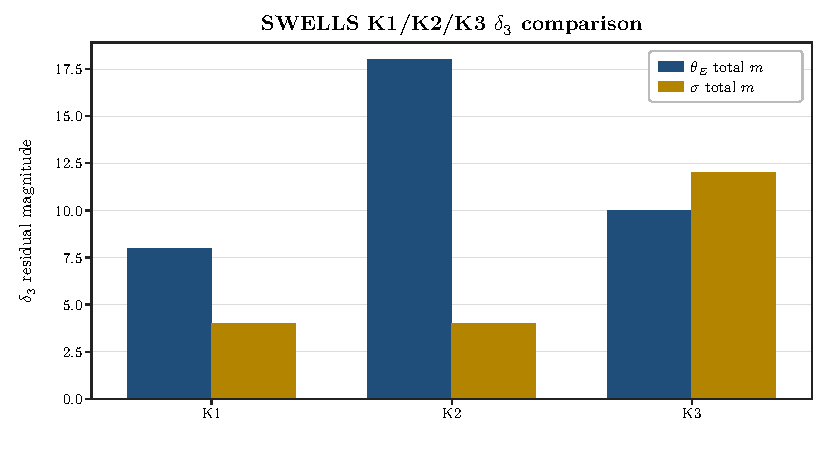
\includegraphics[width=0.92\linewidth,height=0.78\textheight,keepaspectratio]{figures/generated/lensing-05-swells-k-comparison-delta3.pdf}
\caption{SWELLS K1/K2/K3 $\delta_3$ comparison. K2/K3 are audit diagnostics with $\delta_3$ comparison tallies.}
\label{fig:manual-lensing-swells-comparison}
\end{figure}

\begin{figure}[H]
\centering
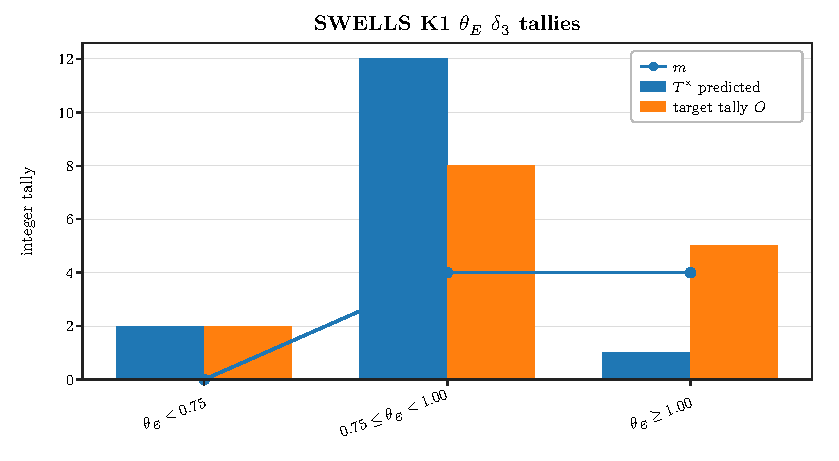
\includegraphics[width=0.92\linewidth,height=0.78\textheight,keepaspectratio]{figures/generated/lensing-06-swells-k1-thetae-delta3-tallies.pdf}
\caption{SWELLS K1 retained-baseline $\theta_E$ $\delta_3$ tallies.}
\label{fig:manual-lensing-swells-k1}
\end{figure}

\subsection{K4 input gate}\label{manual:lensing-k4-input-gate}

K4 is the higher-resolution lensing input-manifest row for independent 3D and time-flow inputs.

% GENERATED FROM typst/manual/tables/k4_3d_timeflow_input_gate_table.typ BY scripts/typ2tex.py (v1.0.0) — DO NOT EDIT.
% Edit canonical Typst under typst/ and regenerate with: python3 scripts/typ2tex.py --root . --outdir latex

\begin{table}[H]
\centering
\caption{K4 independent 3D + time-flow input gate.}
\label{tab:manual-lensing-k4-gate}
{\footnotesize
\begin{tabular}{>{\raggedright\arraybackslash}p{0.160\linewidth}>{\raggedright\arraybackslash}p{0.320\linewidth}>{\raggedright\arraybackslash}p{0.210\linewidth}>{\raggedright\arraybackslash}p{0.150\linewidth}}
\toprule
Input group & Required field & Source status & Gate \\
\midrule
3D density fields & stellar density $\rho_{\star}(R,z,\theta)$ & external / 3D proxy & required \\
3D density fields & gas density $\rho_{\mathrm{gas}}(R,z,\theta)$ & external / 3D proxy & required \\
velocity and flow fields & gas and stellar velocity vector field & IFU / H I / H$\alpha$ & required \\
velocity and flow fields & line-of-sight flow and bobbing/slosh phase & time / kinematic proxy & required \\
momentum fields & angular momentum and radial/linear momentum & independent kinematics & required \\
time-window state & duration/cadence windows for flow transfer & declared pre-score & required \\
lensing target side & image-position bins & quarantined target & required \\
lensing target side & Einstein-radius bins and image count classes & quarantined target & required \\
audit controls & null / permutation controls & declared pre-score & required \\
\bottomrule
\end{tabular}
}
\end{table}


\begin{figure}[H]
\centering
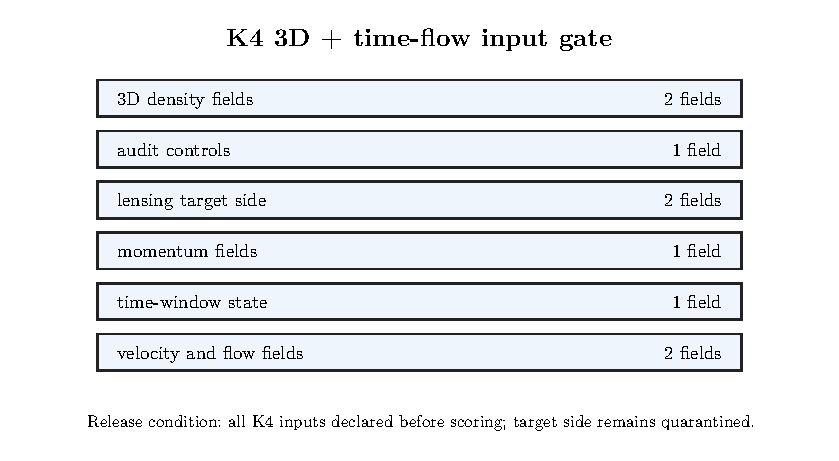
\includegraphics[width=0.92\linewidth,height=0.78\textheight,keepaspectratio]{figures/generated/lensing-07-k4-3d-timeflow-input-gate.pdf}
\caption{K4 higher-resolution lensing data-support gate. The L3 input package records independent 3D + time-flow medium data before the target side joins.}
\label{fig:manual-lensing-k4-gate}
\end{figure}

\subsection{Target-side quarantine and release gate}\label{manual:lensing-release-gate}

A derived $\sigma_{\mathrm{SIE}}$ shares the Einstein radius and distance
inputs of its target construction. Its derivation, source assumptions and
covariance/likelihood must travel with those inputs; it is not an independent
medium measurement. The lensing application next needs per-system
input/output and gate records that regenerate the K0/K1 cohort denominators.
Aggregate agreement alone does not supply that evaluator.

The A$\Omega$ input side carries medium fields, gate values, and declared prediction values. The target side carries image-position, Einstein-radius, and image-count targets after prediction values freeze.

\begin{figure}[H]
\centering
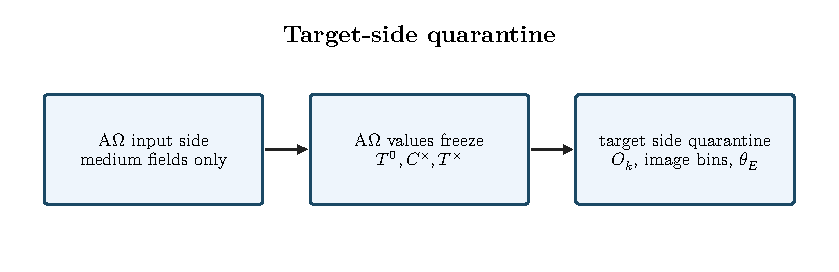
\includegraphics[width=0.92\linewidth,height=0.78\textheight,keepaspectratio]{figures/generated/lensing-08-target-quarantine.pdf}
\caption{Target-side quarantine. A$\Omega$ values freeze before target tallies join.}
\label{fig:manual-lensing-target-quarantine}
\end{figure}

\begin{figure}[H]
\centering
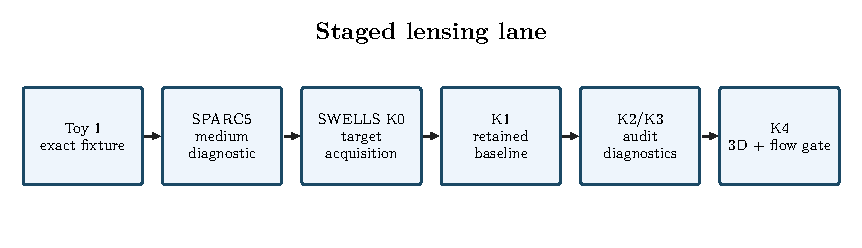
\includegraphics[width=0.92\linewidth,height=0.78\textheight,keepaspectratio]{figures/generated/lensing-09-staged-lensing-lane.pdf}
\caption{Staged galactic lensing lane. Toy fixtures, SPARC5 diagnostics, SWELLS acquisition, retained baseline, K2/K3 audit diagnostics, and K4 gate are kept distinct.}
\label{fig:manual-lensing-staged-lane}
\end{figure}

\begin{figure}[H]
\centering
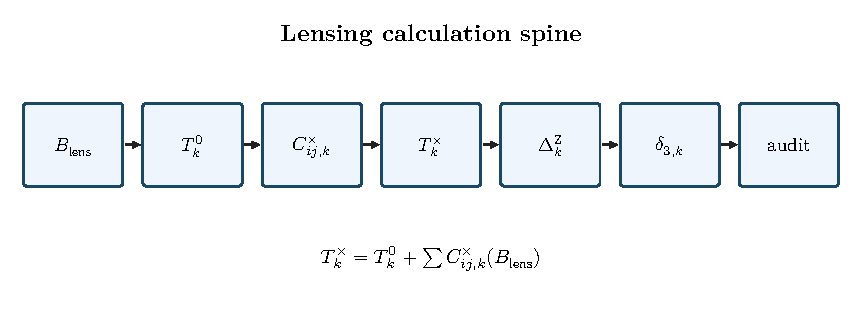
\includegraphics[width=0.92\linewidth,height=0.78\textheight,keepaspectratio]{figures/generated/lensing-10-lensing-calculation-spine.pdf}
\caption{Galactic lensing calculation spine. The $U$-projection and lensing targets remain downstream of declared field-ring values.}
\label{fig:manual-lensing-calculation-spine}
\end{figure}

A completed L3 lensing record carries declared medium fields, declared radiation-current gates, declared target-side quarantine, computed $T^0$, $C^{\times}$, and $T^{\times}$, declared $\lambda_{\mathrm{lens}}$, $\delta_3$ residual table, null controls, audit, and lens residuals after A$\Omega$ values freeze.

\subsection{Five-boundary concentric lens-shell chiral ray D.E.C. walk}\label{manual:lensing:dec-chiral-ray-walk}

\paragraph{Setup and engine verification (\texttt{RC-042}, \texttt{RC-020}).}
Declare the five-boundary lensing stack separating internal FRG cross-shell totals and chiral flips from quarantined SWELLS target acquisition:

\[
B_{\mathrm{src}}\to B_{\mathrm{shell},k}\to B_{\mathrm{FRG}}\to B_{\delta_3}\to B_{\mathrm{SWELLS}}.
\]

Vector \texttt{RC-042} (\texttt{dec\_lensing\_ray\_chiral\_delta3})---archived in \texttt{manual/data/boundary\_sadar/lensing\_ray\_chiral\_dec\_walk.csv} and verified alongside \texttt{RC-020} by \texttt{python3 -B -m manual.engine --sector boundary\_sadar} and \texttt{aod-core --verify-vectors --check-zero-float}---executes the four-shell grazing ray walk ($k=1\dots4$): every shell satisfies the exact Fractal Field Ring Gate identity $T_k^{\times}-T_k^0=C_k^{\times}$ ($7-4=3$, $11-6=5$, $3-5=-2$, $12-8=4$; $\sum_kT_k^{\times}=33$), three active hinge encounters ($k=1,2,4$) flip ray chirality $+1\to-1\to+1\to-1$ while shell $k=3$ preserves $+1$, comparator $O_k=(7,10,3,11)$ yields $\Delta_Z=(0,1,0,1)$ ($\sum m=2$), and $L3/K4$ 3D+time-flow inputs remain explicitly held at $B_{\mathrm{SWELLS}}$ (\texttt{target\_quarantined\_before\_freeze = 1}) until bound.

\begin{figure}[H]
\centering
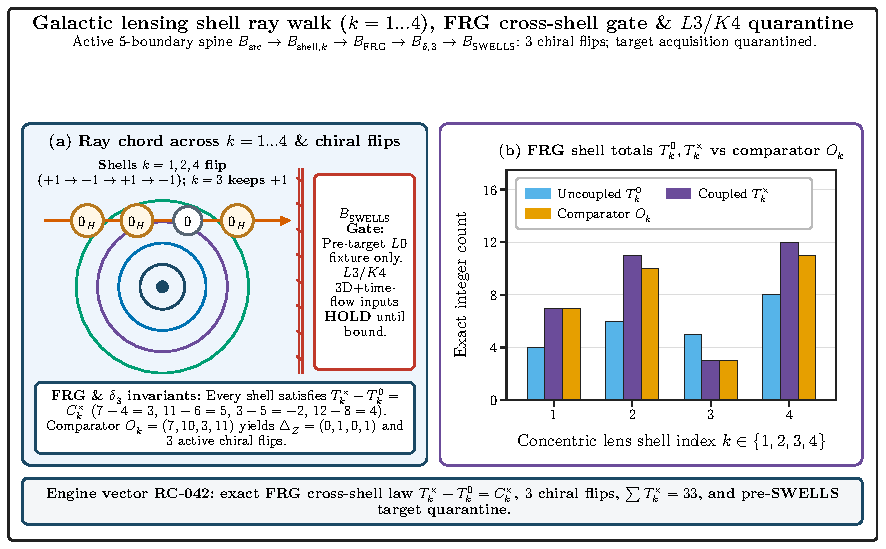
\includegraphics[width=0.92\linewidth,height=0.78\textheight,keepaspectratio]{figures/generated/lensing-ray-boundary-feynman.pdf}
\caption{Grazing ray walk across concentric lens shells $k=1\dots4$, active chiral-flip vertices $0_H$, exact FRG totals $T_k^0,T_k^{\times}$ versus comparator $O_k$, and pre-SWELLS target quarantine (\texttt{RC-042}, \texttt{lensing\_ray\_chiral\_dec\_walk.csv}).}
\label{fig:manual-lensing-ray-boundary-feynman}
\end{figure}

\begin{table}[H]
\centering
\caption{Engine-bound four-shell galactic lensing FRG cross-return and chiral-flip D.E.C. ledger (\texttt{RC-042}, live from \texttt{lensing\_ray\_chiral\_dec\_walk.csv}).}
\label{tab:manual-lensing-dec-ray-walk}
{\footnotesize
\begin{tabular}{>{\raggedleft\arraybackslash}p{0.088\linewidth}>{\raggedleft\arraybackslash}p{0.072\linewidth}>{\raggedleft\arraybackslash}p{0.080\linewidth}>{\raggedleft\arraybackslash}p{0.080\linewidth}>{\raggedleft\arraybackslash}p{0.072\linewidth}>{\raggedleft\arraybackslash}p{0.088\linewidth}>{\raggedleft\arraybackslash}p{0.072\linewidth}>{\raggedleft\arraybackslash}p{0.080\linewidth}>{\centering\arraybackslash}p{0.168\linewidth}}
\toprule
Shell $k$ & $T_k^0$ & $C_k^{\times}$ & $T_k^{\times}$ & Flip & Post $\chi$ & $O_k$ & $\Delta_Z$ & $\delta_3(T_k^{\times},O_k)$ \\
\midrule
1 & 4 & 3 & 7 & 1 & $-$1 & 7 & 0 & (0, 0) \\
2 & 6 & 5 & 11 & 1 & +1 & 10 & 1 & (1, 1) \\
3 & 5 & $-$2 & 3 & 0 & +1 & 3 & 0 & (0, 0) \\
4 & 8 & 4 & 12 & 1 & $-$1 & 11 & 1 & (1, 1) \\
\bottomrule
\end{tabular}
}
\end{table}
